
\documentclass[a4paper,11pt]{article}
\usepackage[a4paper, margin=8em]{geometry}

% usa i pacchetti per la scrittura in italiano
\usepackage[french,italian]{babel}
\usepackage[T1]{fontenc}
\usepackage[utf8]{inputenc}
\frenchspacing 

% usa i pacchetti per la formattazione matematica
\usepackage{amsmath, amssymb, amsthm, amsfonts}

% usa altri pacchetti
\usepackage{gensymb}
\usepackage{hyperref}
\usepackage{standalone}

\usepackage{colortbl}

\usepackage{xstring}
\usepackage{karnaugh-map}

% imposta il titolo
\title{Appunti Calcolatori Elettronici}
\author{Luca Seggiani}
\date{2025}

% imposta lo stile
% usa helvetica
\usepackage[scaled]{helvet}
% usa palatino
\usepackage{palatino}
% usa un font monospazio guardabile
\usepackage{lmodern}

\renewcommand{\rmdefault}{ppl}
\renewcommand{\sfdefault}{phv}
\renewcommand{\ttdefault}{lmtt}

% circuiti
\usepackage{circuitikz}
\usetikzlibrary{babel}

% testo cerchiato
\newcommand*\circled[1]{\tikz[baseline=(char.base)]{
            \node[shape=circle,draw,inner sep=2pt] (char) {#1};}}

% disponi il titolo
\makeatletter
\renewcommand{\maketitle} {
	\begin{center} 
		\begin{minipage}[t]{.8\textwidth}
			\textsf{\huge\bfseries \@title} 
		\end{minipage}%
		\begin{minipage}[t]{.2\textwidth}
			\raggedleft \vspace{-1.65em}
			\textsf{\small \@author} \vfill
			\textsf{\small \@date}
		\end{minipage}
		\par
	\end{center}

	\thispagestyle{empty}
	\pagestyle{fancy}
}
\makeatother

% disponi teoremi
\usepackage{tcolorbox}
\newtcolorbox[auto counter, number within=section]{theorem}[2][]{%
	colback=blue!10, 
	colframe=blue!40!black, 
	sharp corners=northwest,
	fonttitle=\sffamily\bfseries, 
	title=Teorema~\thetcbcounter: #2, 
	#1
}

% disponi definizioni
\newtcolorbox[auto counter, number within=section]{definition}[2][]{%
	colback=red!10,
	colframe=red!40!black,
	sharp corners=northwest,
	fonttitle=\sffamily\bfseries,
	title=Definizione~\thetcbcounter: #2,
	#1
}

% disponi codice
\usepackage{listings}
\usepackage[table]{xcolor}

\definecolor{codegreen}{rgb}{0,0.6,0}
\definecolor{codegray}{rgb}{0.5,0.5,0.5}
\definecolor{codepurple}{rgb}{0.58,0,0.82}
\definecolor{backcolour}{rgb}{0.95,0.95,0.92}

\lstdefinestyle{codestyle}{
		backgroundcolor=\color{black!5}, 
		commentstyle=\color{codegreen},
		keywordstyle=\bfseries\color{magenta},
		numberstyle=\sffamily\tiny\color{black!60},
		stringstyle=\color{green!50!black},
		basicstyle=\ttfamily\footnotesize,
		breakatwhitespace=false,         
		breaklines=true,                 
		captionpos=b,                    
		keepspaces=true,                 
		numbers=left,                    
		numbersep=5pt,                  
		showspaces=false,                
		showstringspaces=false,
		showtabs=false,                  
		tabsize=2
}

\lstdefinestyle{shellstyle}{
		backgroundcolor=\color{black!5}, 
		basicstyle=\ttfamily\footnotesize\color{black}, 
		commentstyle=\color{black}, 
		keywordstyle=\color{black},
		numberstyle=\color{black!5},
		stringstyle=\color{black}, 
		showspaces=false,
		showstringspaces=false, 
		showtabs=false, 
		tabsize=2, 
		numbers=none, 
		breaklines=true
}


\lstdefinelanguage{assembler}{ 
  keywords={AAA, AAD, AAM, AAS, ADC, ADCB, ADCW, ADCL, ADD, ADDB, ADDW, ADDL, AND, ANDB, ANDW, ANDL,
        ARPL, BOUND, BSF, BSFL, BSFW, BSR, BSRL, BSRW, BSWAP, BT, BTC, BTCB, BTCW, BTCL, BTR, 
        BTRB, BTRW, BTRL, BTS, BTSB, BTSW, BTSL, CALL, CBW, CDQ, CLC, CLD, CLI, CLTS, CMC, CMP,
        CMPB, CMPW, CMPL, CMPS, CMPSB, CMPSD, CMPSW, CMPXCHG, CMPXCHGB, CMPXCHGW, CMPXCHGL,
        CMPXCHG8B, CPUID, CWDE, DAA, DAS, DEC, DECB, DECW, DECL, DIV, DIVB, DIVW, DIVL, ENTER,
        HLT, IDIV, IDIVB, IDIVW, IDIVL, IMUL, IMULB, IMULW, IMULL, IN, INB, INW, INL, INC, INCB,
        INCW, INCL, INS, INSB, INSD, INSW, INT, INT3, INTO, INVD, INVLPG, IRET, IRETD, JA, JAE,
        JB, JBE, JC, JCXZ, JE, JECXZ, JG, JGE, JL, JLE, JMP, JNA, JNAE, JNB, JNBE, JNC, JNE, JNG,
        JNGE, JNL, JNLE, JNO, JNP, JNS, JNZ, JO, JP, JPE, JPO, JS, JZ, LAHF, LAR, LCALL, LDS,
        LEA, LEAVE, LES, LFS, LGDT, LGS, LIDT, LMSW, LOCK, LODSB, LODSD, LODSW, LOOP, LOOPE,
        LOOPNE, LSL, LSS, LTR, MOV, MOVB, MOVW, MOVL, MOVSB, MOVSD, MOVSW, MOVSX, MOVSXB,
        MOVSXW, MOVSXL, MOVZX, MOVZXB, MOVZXW, MOVZXL, MUL, MULB, MULW, MULL, NEG, NEGB, NEGW,
        NEGL, NOP, NOT, NOTB, NOTW, NOTL, OR, ORB, ORW, ORL, OUT, OUTB, OUTW, OUTL, OUTSB, OUTSD,
        OUTSW, POP, POPL, POPW, POPB, POPA, POPAD, POPF, POPFD, PUSH, PUSHL, PUSHW, PUSHB, PUSHA, 
				PUSHAD, PUSHF, PUSHFD, RCL, RCLB, RCLW, MOVSL, MOVSB, MOVSW, STOSL, STOSB, STOSW, LODSB, LODSW,
				LODSL, INSB, INSW, INSL, OUTSB, OUTSL, OUTSW
        RCLL, RCR, RCRB, RCRW, RCRL, RDMSR, RDPMC, RDTSC, REP, REPE, REPNE, RET, ROL, ROLB, ROLW,
        ROLL, ROR, RORB, RORW, RORL, SAHF, SAL, SALB, SALW, SALL, SAR, SARB, SARW, SARL, SBB,
        SBBB, SBBW, SBBL, SCASB, SCASD, SCASW, SETA, SETAE, SETB, SETBE, SETC, SETE, SETG, SETGE,
        SETL, SETLE, SETNA, SETNAE, SETNB, SETNBE, SETNC, SETNE, SETNG, SETNGE, SETNL, SETNLE,
        SETNO, SETNP, SETNS, SETNZ, SETO, SETP, SETPE, SETPO, SETS, SETZ, SGDT, SHL, SHLB, SHLW,
        SHLL, SHLD, SHR, SHRB, SHRW, SHRL, SHRD, SIDT, SLDT, SMSW, STC, STD, STI, STOSB, STOSD,
        STOSW, STR, SUB, SUBB, SUBW, SUBL, TEST, TESTB, TESTW, TESTL, VERR, VERW, WAIT, WBINVD,
        XADD, XADDB, XADDW, XADDL, XCHG, XCHGB, XCHGW, XCHGL, XLAT, XLATB, XOR, XORB, XORW, XORL},
  keywordstyle=\color{blue}\bfseries,
  ndkeywordstyle=\color{darkgray}\bfseries,
  identifierstyle=\color{black},
  sensitive=false,
  comment=[l]{\#},
  morecomment=[s]{/*}{*/},
  commentstyle=\color{purple}\ttfamily,
  stringstyle=\color{red}\ttfamily,
  morestring=[b]',
  morestring=[b]"
}

\lstset{language=assembler, style=codestyle}

% disponi sezioni
\usepackage{titlesec}

\titleformat{\section}
	{\sffamily\Large\bfseries} 
	{\thesection}{1em}{} 
\titleformat{\subsection}
	{\sffamily\large\bfseries}   
	{\thesubsection}{1em}{} 
\titleformat{\subsubsection}
	{\sffamily\normalsize\bfseries} 
	{\thesubsubsection}{1em}{}

% tikz
\usepackage{tikz}

% float
\usepackage{float}

% grafici
\usepackage{pgfplots}
\pgfplotsset{width=10cm,compat=1.9}

% disponi alberi
\usepackage{forest}

\forestset{
	rectstyle/.style={
		for tree={rectangle,draw,font=\large\sffamily}
	},
	roundstyle/.style={
		for tree={circle,draw,font=\large}
	}
}

% disponi algoritmi
\usepackage{algorithm}
\usepackage{algorithmic}
\makeatletter
\renewcommand{\ALG@name}{Algoritmo}
\makeatother

% disponi numeri di pagina
\usepackage{fancyhdr}
\fancyhf{} 
\fancyfoot[L]{\sffamily{\thepage}}

\makeatletter
\fancyhead[L]{\raisebox{1ex}[0pt][0pt]{\sffamily{\@title \ \@date}}} 
\fancyhead[R]{\raisebox{1ex}[0pt][0pt]{\sffamily{\@author}}}
\makeatother

\begin{document}
% sezione (data)
\section{Lezione del 01-04-25}

% stili pagina
\thispagestyle{empty}
\pagestyle{fancy}

% testo
Riprendiamo la trattazione dei moduli MMU.
Eravamo partiti dalla S-MMU, che prendevamo solo come esempio funzionale, e avevamo in seguito introdotto la T-MMU, che sfrutta una struttura dati ad albero (la \textit{trie}) per mantenere in aniera più efficiente le associazioni pagina-frame.
Passiamo adesso alla descrizione della \textbf{MMU} vera e propria, senza le semplificazioni che avevamo assunto per la S-MMU e la T-MMU.

\subsubsection{MMU Reale}
Abbiamo che le tabelle della MMU stanno in RAM, assieme ai dati stessi cui la MMU vuole accedere.
La struttura \textit{trie} sta quindi in memoria, e l'MMU è dotata di un registro \textbf{CR3} che mantiene la posizione della prima tabella (avevamo visto, quella di livello 4). 
Il processore si occupa quindi di creare la trie, e di fornirne l'indirizzo alla MMU, su tale registro.

Notiamo che gli indirizzi che stanno nelle tabelle della MMU, che sono comunque in memoria, sono indirizzi \textit{fisici}, e anzi il contenuto dello stesso registro CR3 è un indirizzo \textit{fisico}.

Perchè il kernel possa accedere a tali indirizzi senza problemi (ricordiamo che tutto ciò che esce dalla CPU è considerato dalla MMU come un indirizzo \textit{virtuale}), si mette tale struttura nella memoria sistema, in modo che gli indirizzi ivi contenuti si traducano in loro stessi.

\subsubsection{Bootstrap della MMU}
Nello specifico, possiamo immaginare che il kernel faccia, all'avvio, le seguenti operazioni:
\begin{enumerate}
	\item Preso lo spazio indirizzabile come diviso in 2 (che abbiamo visto essere il caso nell'architettura x86\_64), dedica una delle due parti (la superiore in Windows, l'inferiore in Linux) alla memoria sistema;
	\item Inizializza un primo trie per la MMU in memoria sistema, e vi crea una serie di pagine (una \textbf{finestra} sulla memoria virtuale, detta \textbf{ªM}), corrispondenti ai loro frame, di tipo sistema, in modo da poter indirizzare la memoria con indirizzi che si traducono in loro stessi;

		# graf. finestra fisica 

	\item Carica tale trie in CR3 ed abilita la MMU.
\end{enumerate}

Da qui in poi il kernel avrà accesso, attraverso tale finestra, all'interezza della memoria fisica mappata con indirizzi fisici (cioè con indirizzi virtuali mappati con l'identità ad indirizzi fisici).

Notiamo di poter tranquillamente creare tale finestra, in quanto in $2^{48}$ possibili indirizzi virtuali mappiamo anche più di una volta tutta la finestra della memoria fisica.

\subsubsection{Translation Lookaside Buffer}
Abbiamo che sfruttando il modello visto finora ogni accesso alla RAM si traduce in realtà a diversi accessi (fino a 5, accesso alle tabelle dal 4 all'1 della trie corrente, e l'accesso all'indirizzo fisico desiderato).

Visto che era proprio la RAM ad essere, come avevamo detto, la parte più lenta del sistema, è necessario introdurre una cache a parte dedicata alla MMU, che viene detta \textbf{TLB}, \textit{Translation Lookaside Buffer}.
Il TLB tiene traccia delle coppie indirizzo virtuale - indirizzo fisico più usate, limitando la necessità dei table walk alle sole istanze dove sono strettamente necessari.

Il TLB è perlopiù trasparente alla CPU.
Esistono istruzioni, però, come la \lstinline|INVLPG|, che permettono di modificare lo stato del TLB.
Questa infatti permette di invalidare un indirizzo virtuale, se questo è contenuto nel TLB (costringendo a un nuovo page walk in fase di ricerca di tale indirizzo).

La struttura del TLB è analoga a quella della cache: si prendono i 48 bit di indirizzo virtuale, di cui i 12 più bassi saranno come sempre l'offset, e si dividono i 36 rimanenti in due parti che usiamo come indice e come numero di pagina in una memoria delle etichette.
Una and fa il bit di validità nella tabella delle entrate e un comparatore fra il numero di pagina e l'etichetta fissata all'indice corrente ci darà quindi gli hit di cache.

\noindent
\begin{minipage}{\textwidth}
La struttura è quindi la seguente:
\begin{center}
	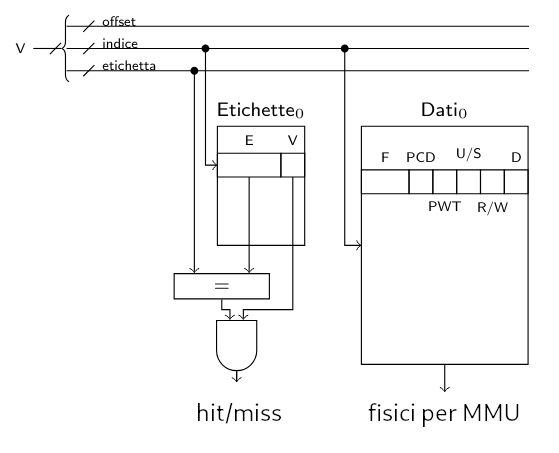
\includegraphics[scale=0.78]{../figures/tlb.png}
\end{center}
\end{minipage}

Dove una memoria a sé stante conterrà quindi gli indirizzi fisici veri e propri, oltre ad alcuni flag.
Notiamo che questa non ha bisogno di conoscere A (se è nel TLB ci è già stato fatto accesso).
Ad esempio però vogliamo sapere PCD e PWT, in quanto questi regoleranno l'accesso o meno via cache.
Abbiamo poi un solo bit dedicato a U/S e R/W, in quanto comunque tutto ciò che vorremo sapere è se a quell'indirizzo si può accedere o meno nel contesto corrente.
Infine, manteniamo il bit D.
Effettuare il write back di tale bit è complicato in quanto occorre effettivamente ritrovare la pagina effettuando il table walk.
Possiamo risolvere questa situazione fingendo di non conoscere (praticamente invalidando) una pagina, anche se conosciuta, quando il suo bit D è basso, costringendo l'MMU ad effettuare il page walk ed alzarlo. 

Notiamo infine di poter applicare tutte le ottimizzazioni che avevamo visto per le cache tradizionali, inclusa l'introduzione di memorie aggiuntive e una memoria per l'LRU, in modo da realizzare effettivamente una cache a contenitori associativi.

\subsubsection{Pagine di grandi dimensioni}
Vediamo un ultimo dettaglio sulla MMU approfondendo il discorso delle pagine di grandi dimensioni (\textit{huge page}).
Anche se teoricamente si potrebbe procedere ignorando questi oggetti, il significato della MMU è quello di mantenere \textit{pagine}, e quindi offset all'interno di tali pagine, e dobbiamo quindi mantenere informazione riguardo al fatto che gli indirizzi in una huge page sono più grandi di quelli in una pagina normale da 4 KiB (come abbiamo riportato in 14.0.3).

Storicamente, trovata una huge page, la MMU la caricava interamente all'interno della cache TLB.
Oggi, si mantengono 3 TLB separati per ogni dimensione di pagina (1 GiB, 2 MiB e 4 KiB).

\end{document}
